\Subhead{2.6.3}{Линзовые линии и открытые резонаторы. Гауссовские пучки}

Параксиальное поле $U=A\e^{\ii kz}$ удовлетворяет $2\ii kA_z+\Delta_\perp A=0$. Фундаментальное осесимметричное решение:
\begin{align}
 U(r,z)&=U_0\frac{w_0}{w(z)}\exp\left[-\frac{r^2}{w^2(z)}\right]
 \exp\left[\ii kz+\ii\frac{kr^2}{2R(z)}-\ii\zeta(z)\right],\\
 w(z)&=w_0\sqrt{1+(z/z_R)^2},\quad z_R=kw_0^2/2,\\
 R(z)&=z[1+(z_R/z)^2],\quad \zeta(z)=\arctan(z/z_R).
\end{align}
$w$ — радиус поля по уровню $1/\e$, интенсивности по $1/\e^2$. Дальняя расходимость полуугла $\theta\simeq\lambda/(\pi w_0)$: малое пятно требует широкого углового спектра.

Комплексный параметр $1/q=1/R+2\ii/(kw^2)$ (при записи поля с $\e^{+\ii kz}$) изменяется через параксиальную систему по правилу $q_2=(Aq_1+B)/(Cq_1+D)$. Линза меняет кривизну, свободный промежуток — размер пучка. В периодической линзовой линии условие сохранения гауссова профиля после ячейки — неподвижная точка этого преобразования с физическим знаком мнимой части. Для вещественной ABCD-матрицы с определителем 1 устойчивость лучей требует $|(A+D)/2|<1$.

Открытый резонатор — повторяющаяся система зеркальных отражений. Для двух сферических зеркал расстояния $L$, $g_j=1-L/R_j$; обычная область устойчивости $0<g_1g_2<1$, границы и вырожденные случаи рассматриваются отдельно. Конфокальный резонатор устойчив, хотя лежит в особой вырожденной точке этой параметризации. Конечные апертуры создают дифракционные потери. Подробный спектр резонатора приведён в вопросе~\Qref{4.2}.
\begin{center}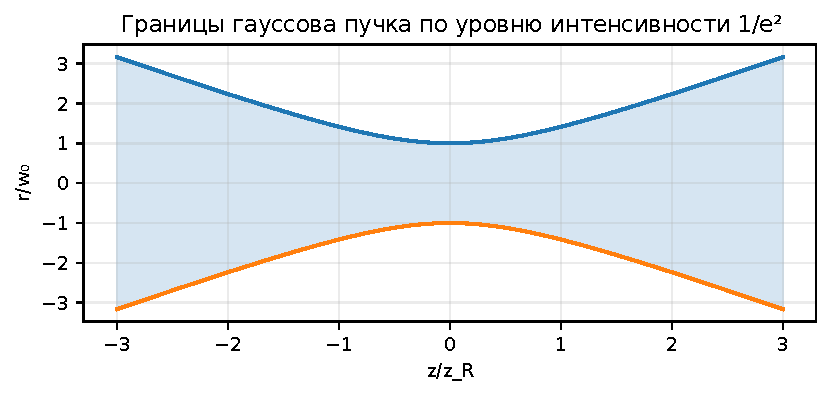
\includegraphics[width=0.8\linewidth]{figures/gaussian.pdf}\end{center}

